\setchapterpreamble[u]{\margintoc}
\chapter{软件层面的准备}
\labch{software}

\setlength\parindent{2em} 本章将介绍本课题中所用到的软件的选择、编译、配置等过程。包括适配该MCU的操作系统的选择、编译;应用程式的编译、配置;对Apple HomeKik的适配等过程。本课题的研究秉承开源的理念,除Apple HomeKit相关项目(商用软件)外,本课题所选择的操作系统、应用程式均为开放源码软件系统。另,本课题中设计的硬件电路等设备也均开源。

\section{适用于微控单元的实时操作系统}

\setlength\parindent{2em} 既然选择ESP01S当作微控单元,一个合适的操作系统是必要的。考虑到这个项目所要实现的功能,一般的嵌入式操作系统是无法应对的,因为它不具有“实时性”这一大特征。换句话说,从事件的发生到操作系统的响应之间的时间应该受到严格的限制,以保证各个任务能够及时地进行。所以我们需要使用“实时操作系统\sidenote[][-0.5cm]{实时操作系统(RTOS)是指当外界事件或数据产生时,能够接受并以足够快的速度予以处理,其处理的结果又能在规定的时间之内来控制生产过程或对处理系统做出快速响应,调度一切可利用的资源完成实时任务,并控制所有实时任务协调一致运行的操作系统。提供及时响应和高可靠性是其主要特点。}”来适配这个项目。

\par 总的来看,目前有许多操作系统可供选择。比如说$\mu$Clinux、$\mu$C/OS-II、embOS、FreeRTOS等等。其中,$\mu$Clinux的结构相对复杂,而且缺少良好的实时性,故这次未采用。另外,$\mu$C/OS-II、embOS等属于商业操作系统,而非开放源码的系统,灵活度、可移植性大大降低,亦不采用。综上,本研究项目选择了FreeRTOS操作系统。

\begin{marginfigure}[-0.5cm]
	
\includegraphics{freertos}
	\caption[freertos]{Logo of FreeRTOS\\
	\url{https://www.freertos.org/}}
\end{marginfigure}


\par FreeRTOS系统——大概是因为开源——有着诸多的移植版本,几乎适配所有平台,ESP01S也有适配。适用于ESP01S的FreeRTOS之一,也就是本项目所采用的,叫做“ESP-OPEN-RTOS”,来自Github开源平台:\\
\url{https://github.com/SuperHouse/esp-open-rtos}。

\section{ESP-OPEN-RTOS的编译}

\setlength\parindent{2em} 根据ESP-OPEN-RTOS位于Github的官方Wiki中,给出了较为具体的编译步骤,难度不算大,与平常编译Android系统或Linux内核差不多。本次使用的编译平台为Intel x86,操作系统为Kali Linux\sidenote{Kali Linux is an open source project that is maintained and funded by Offensive Security, a provider of world-class information security training and penetration testing services.}。由于Kali Linux中内置较为完整的Linux开发环境,故使用其作为编译主机。编译步骤大致如下:

\begin{marginfigure}[0cm]
	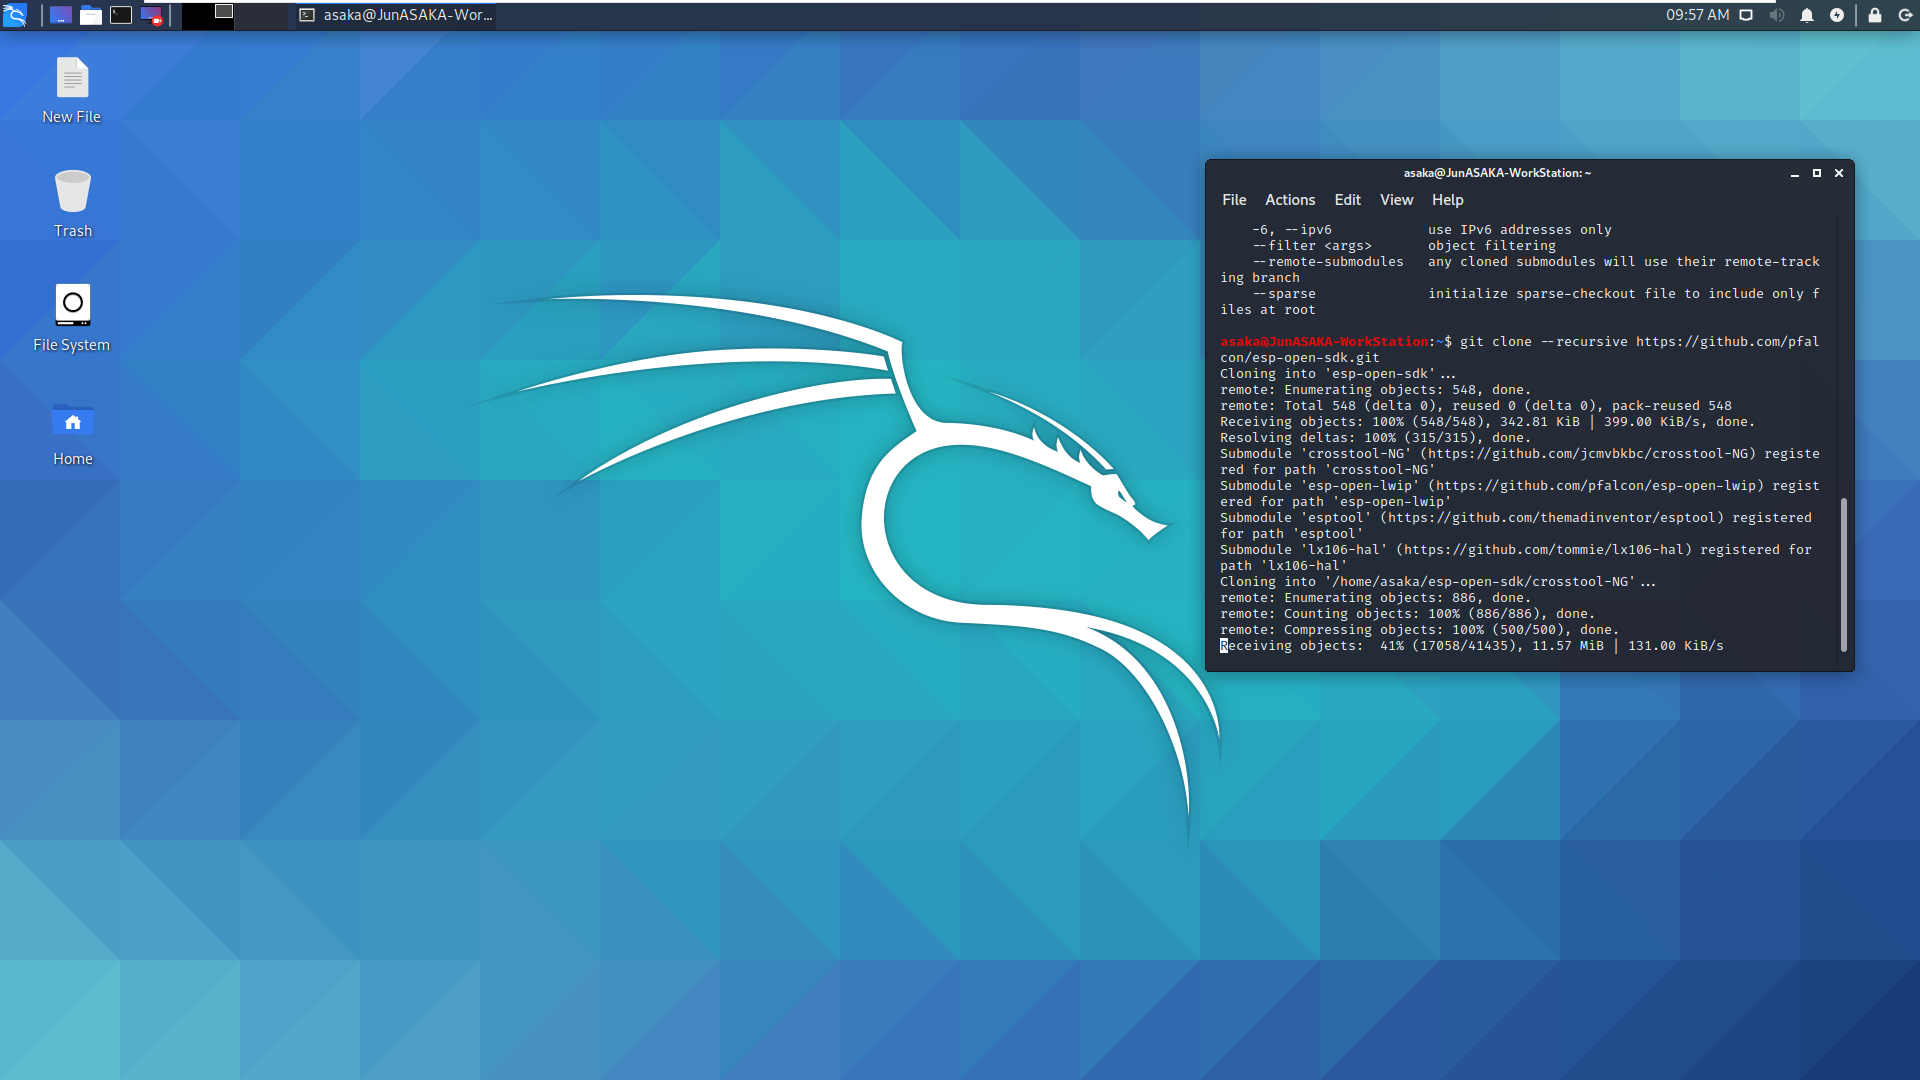
\includegraphics{clone}
	\caption[clone]{RTOS的编译过程}
\end{marginfigure}


\begin{itemize}
	\item 配置适用于ESP的SDK,包括下载SDK源代码并编译适用于主机的二进制文件。
	\item 安装预编译的esptool
	\item 从GitHub克隆源代码
	\item 修改头文件中关于无线网络的配置
	\item 修改其他配置文件
	\item 编译可引导的二进制文件
	\item 烧录(这一步放在后面进行)
\end{itemize}

最后根据Wiki,得到如图\reffig{normalrtosbin}两个二进制文件。

\begin{figure*}[h!]
	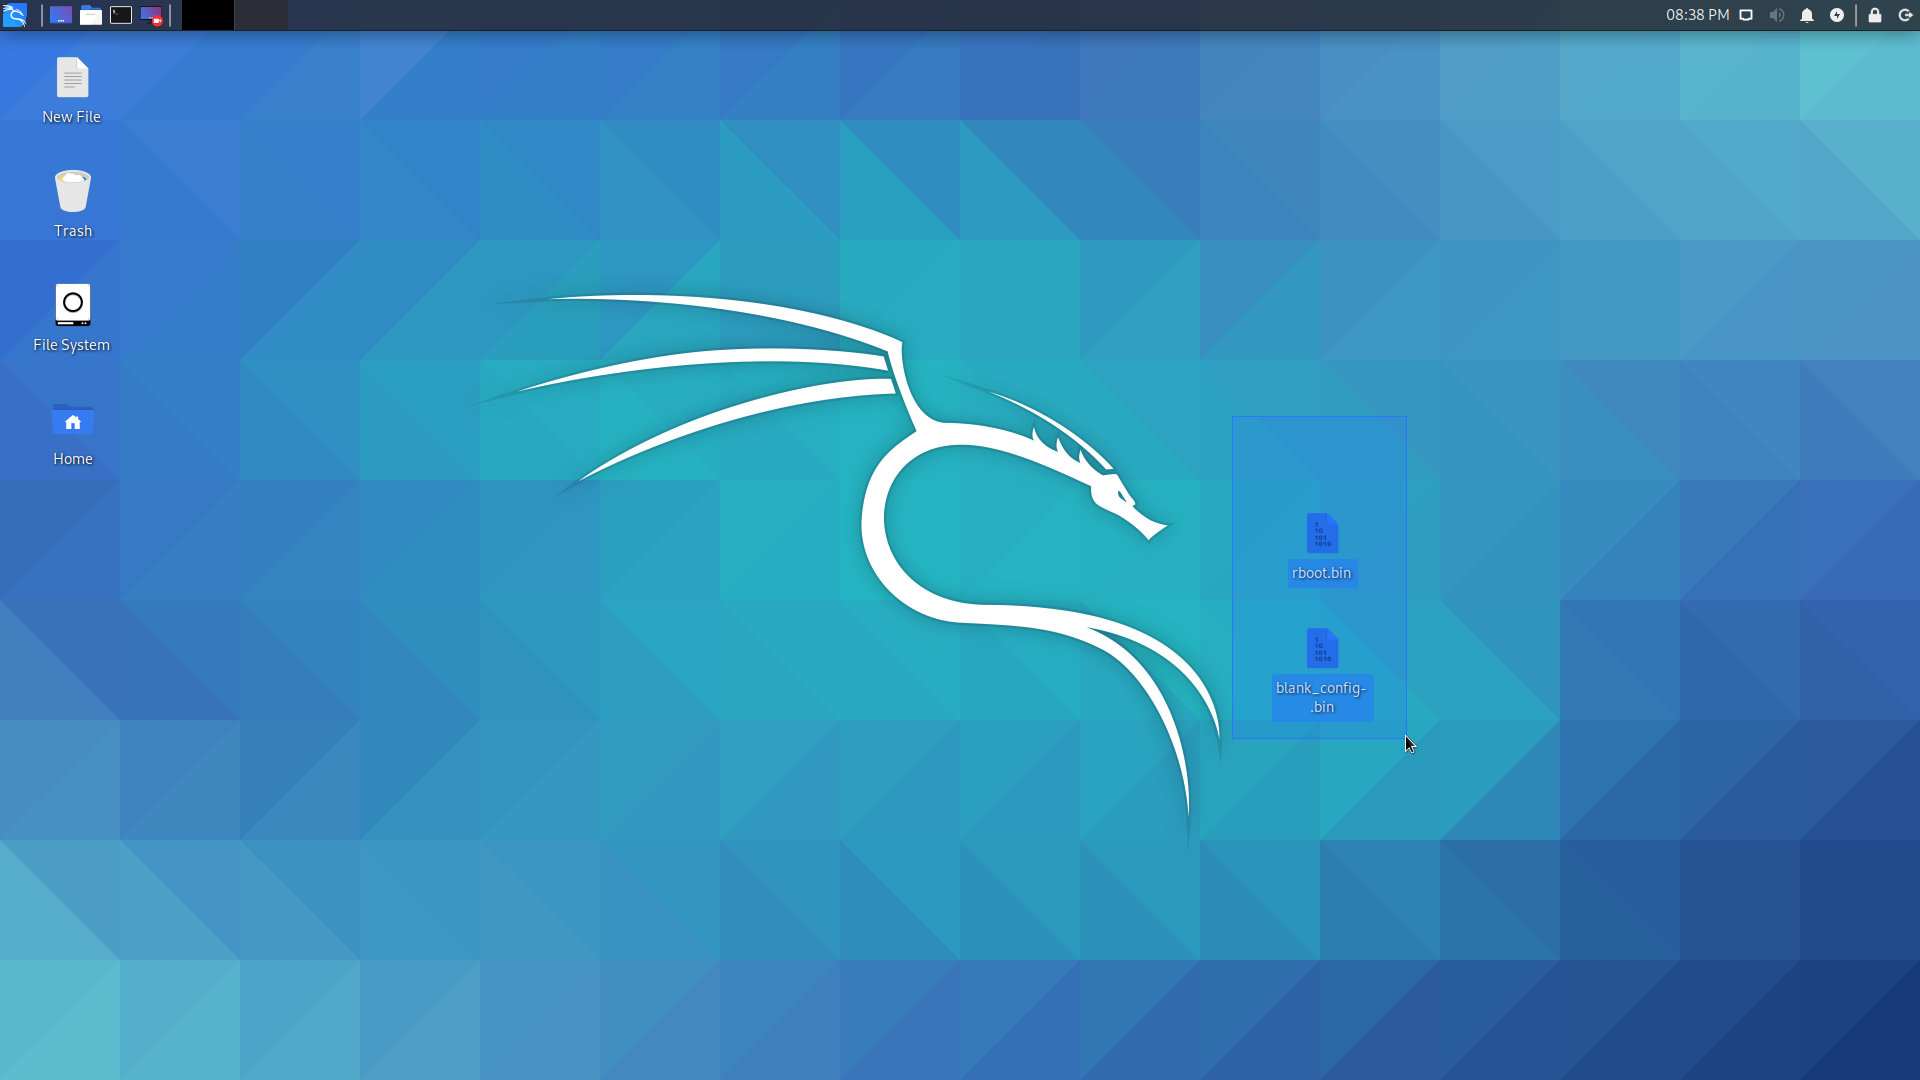
\includegraphics[width=\textwidth]{rtosbin}
	\caption[rtosbin]{编译得到的两个二进制文件}
	\labfig{normalrtosbin}
\end{figure*}

\section{适配于ESP01S以支持Apple HomeKit的应用程式}

\setlength\parindent{2em} 根据Apple Inc.给出的HomeKit Accessory Protocol Specification Non-commercial version\sidenote{\url{https://developer.apple.com/homekit/specification/}},HAP协议是Apple发布的用于Apple智能设备控制物联网智能家居的通讯协议,包含BLE和IP两种方式。为此,本研究项目需要一个适配于ESP01S以让其支持Apple HomeKit通讯协议的应用程式。

\par 在Github上可以找到许多支持HAP的应用程式;其中,本次选择了Home Accessory Architect(以下简称HAA):\url{https://github.com/RavenSystem/esp-homekit-devices}。这次的编译相对来说更简单,仍然需要用到ESP-OPEN-SDK,就像编译RTOS一样;主机操作系统仍是Kali Linux。编译步骤大致如下:

\begin{marginfigure}[0cm]
	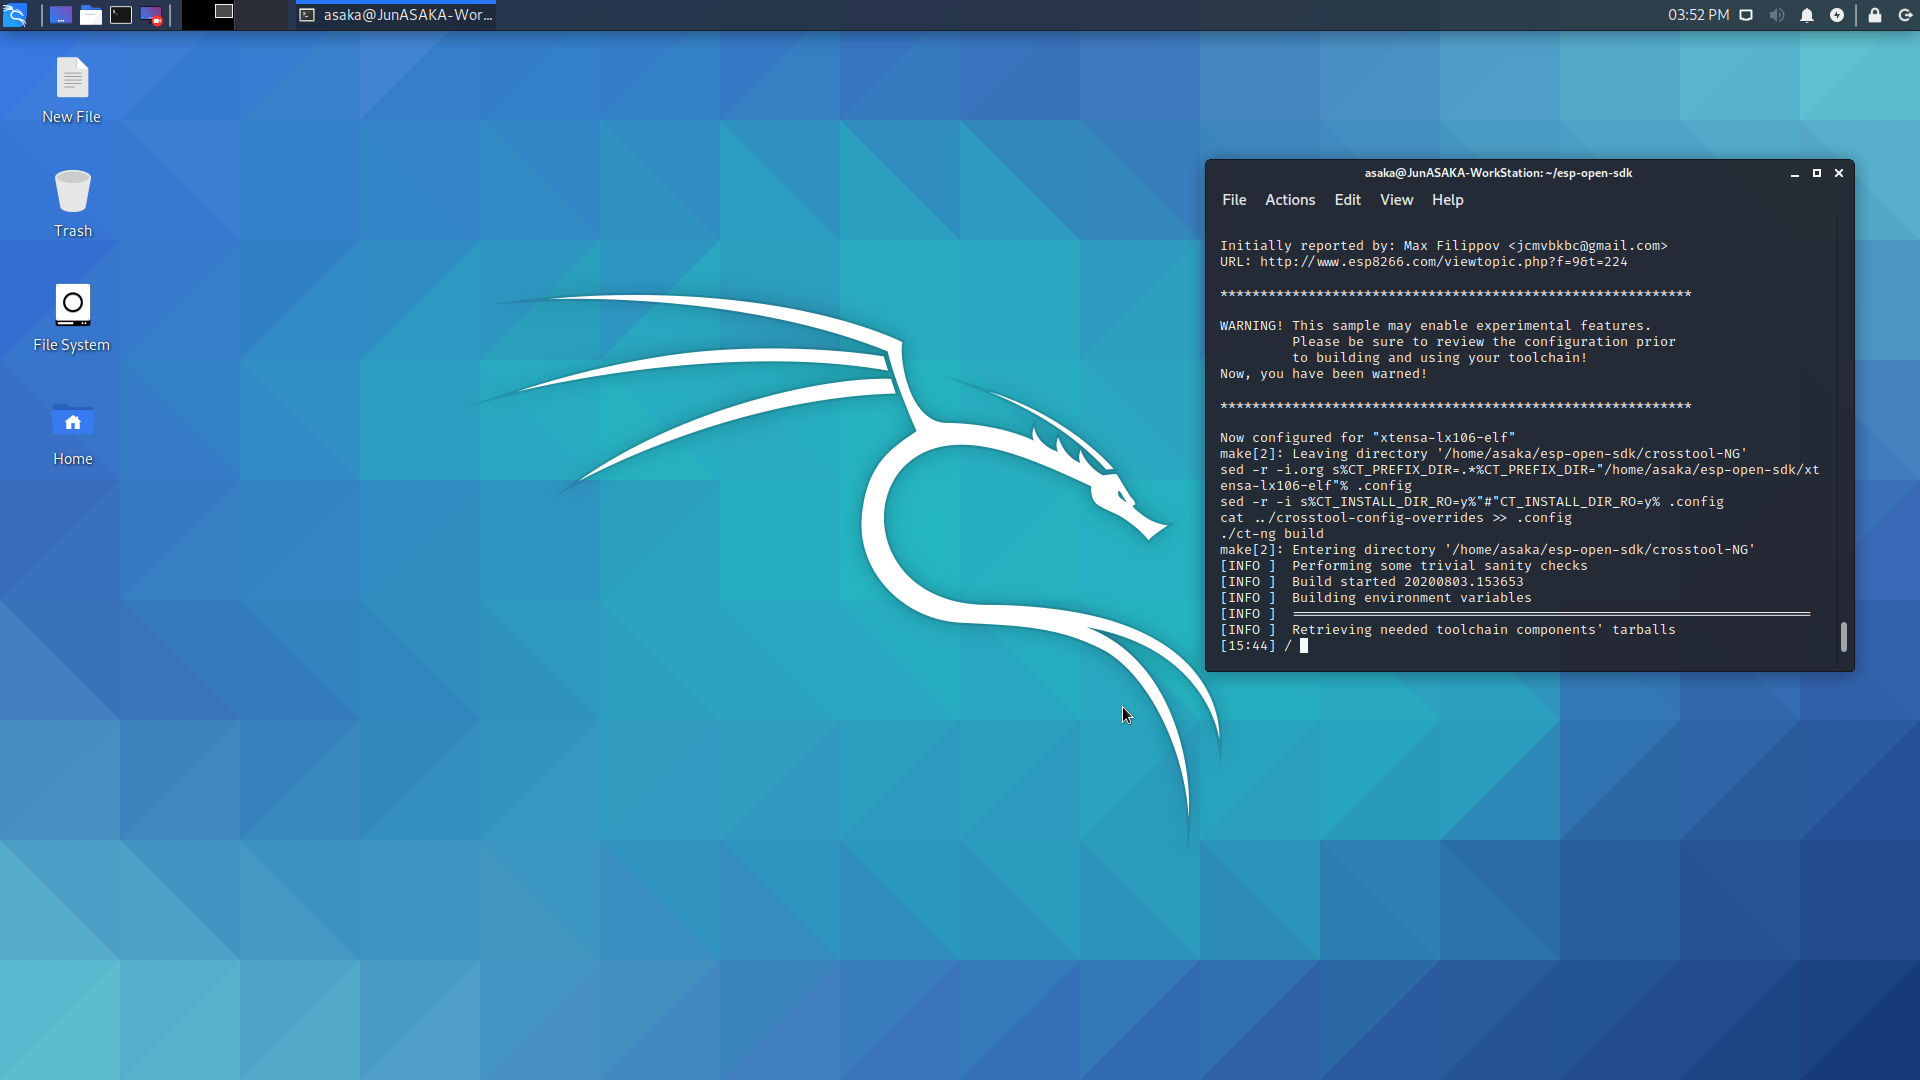
\includegraphics{build}
	\caption[build]{RTOS的编译过程}
\end{marginfigure}

\begin{itemize}
	\item 配置适用于ESP的SDK,上次编译时已经完成了。
	\item 从GitHub克隆源代码
	\item 编译可引导的二进制文件
	\item 安装与配置(这一步放在后面进行)
\end{itemize}

最后得到一个二进制文件。至此,总共编译完成了三个二进制文件如图\reffig{normalbin},包括操作系统和应用程式。接下来将介绍将它们烧录到微控单元并配置的过程。

\begin{figure*}[h!]
	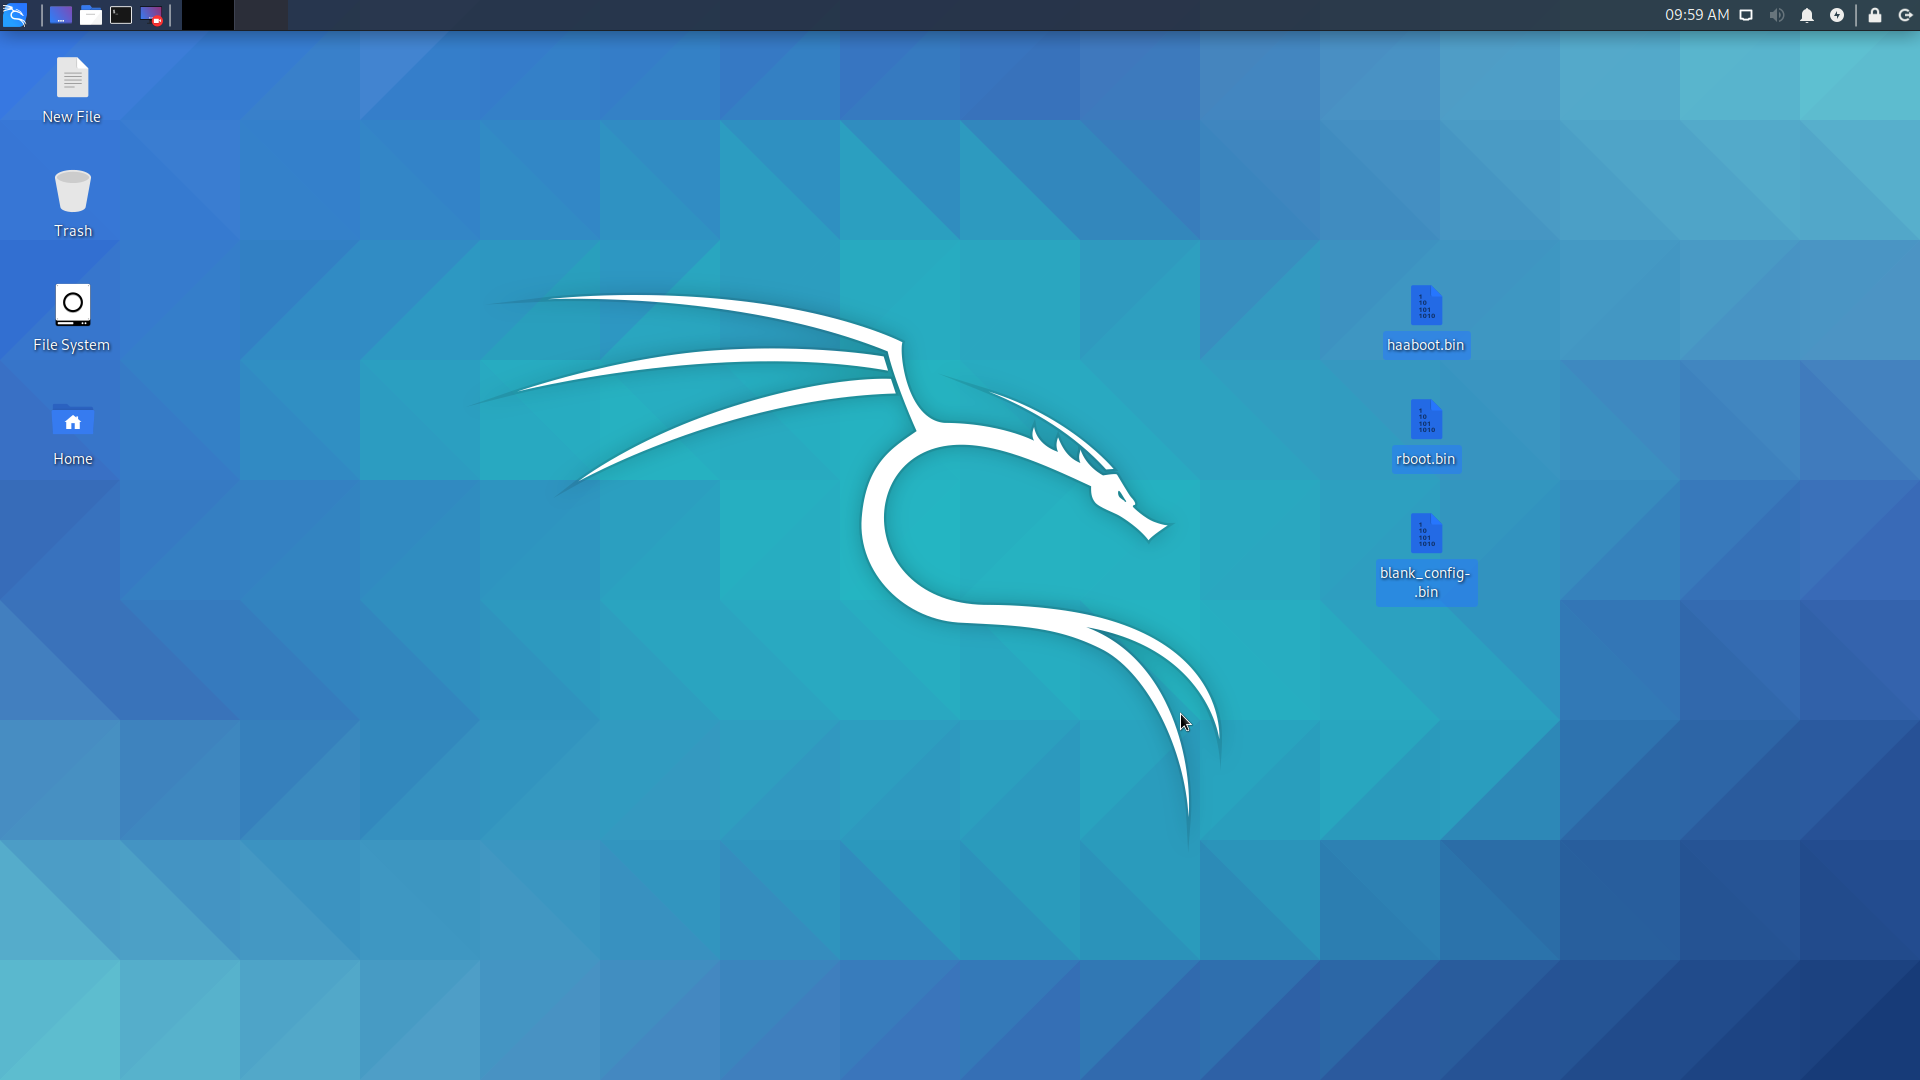
\includegraphics[width=\textwidth]{bin}
	\caption[bin]{所需所有的二进制文件}
	\labfig{normalbin}
\end{figure*}
